\chapter{Triplanar-Net}
\label{chapter5}
\todo{Aim for 5 to 6 pages}

It is computationally demanding to work with three-dimensional volumetric data, and consequently with three-dimensional neural networks (such as the ones shown in chapter \ref{chapter4}); this applies even more so for the case of aneurysm segmentation where localization is difficult due to the size of aneurysms. This could be overcome by using low-resolution data or by using shallow networks, however this would adversely affect performance. Therefore the proposed network architecture works with 2D projections of patches of the volumetric data. Since we are working with cerebral TOF-MRAs for the task of aneurysm segmentation, the projections used are axial, coronal and sagittal Maximum Intensity Projections (MIPs). 

To obtain better 3D context, 3D reconstruction using the orthogonal views is carried out within the network and the network is trained on 3D labels. This removes the need to naively reconstruct the label after obtaining 2D labels, and also allows the network to learn 3D context while still being lightweight and non-resource intensive. 

The design of the input arms is heavily inspired by the BtrflyNet architecture, but deeper and with three input arms for the three MIPs \cite{sekuboyina2018}. \todo{Talk about conv operations in input path} \todo{Talk about 3D reconstruction} \todo{Talk about 3D upsampling conv operations}. \todo{Talk about number of parameters?}


\section{Maximum Intensity Projection}
Maximum Intensity Projection is a method that consists of projecting the voxel with the highest intensity lying in the direction of the plane of projection. It allows representing three-dimensional objects in two dimensions. MIPs have several advantages: vascular structures are well defined and appear clearly as tubular branching structures, the susceptibility to noise is highly reduced due to projecting only the maximum value across a view, and through MIP the use of two dimensional images immensely reduces required resources and parameters. Figure \ref{fig:mip} show axial, coronal and sagittal MIPs obtained from two positive cases in the dataset. 

\begin{figure}[h]
	\centering
	\begin{subfigure}{\linewidth}
		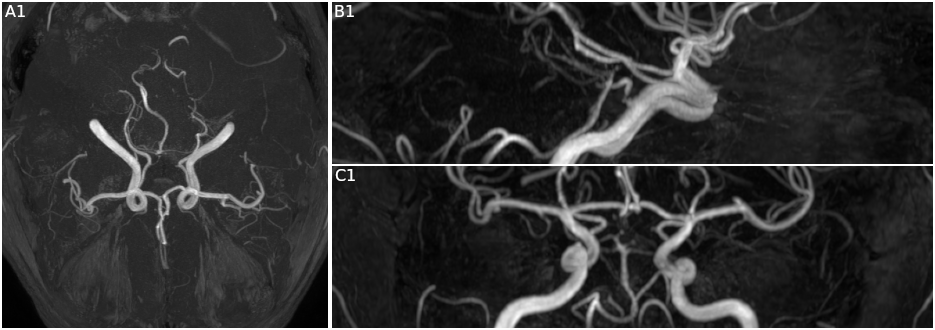
\includegraphics[width=\linewidth]{figures/mip_10021.png}
%		\phantomsubcaption
%		\label{fig:mip_10021.png}
	\end{subfigure}
	\begin{subfigure}{\linewidth}
		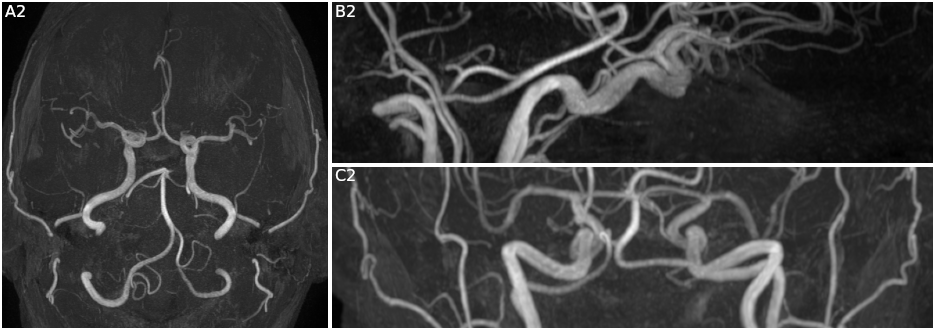
\includegraphics[width=\linewidth]{figures/mip_10028.png}
%		\phantomsubcaption
%		\label{fig:mip_10028.png}
	\end{subfigure}
	\caption[Maximum Intensity Projections of two positive cases.]{\todo{caption}}
	\label{fig:mip}
\end{figure}

\begin{figure}[t]
	\centering
	\begin{subfigure}{\linewidth}
		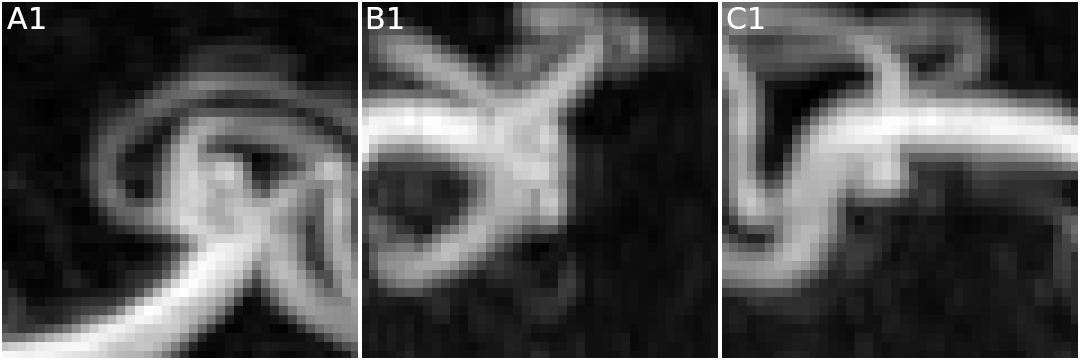
\includegraphics[width=\linewidth]{figures/mip_patch10021.png}
	\end{subfigure}
	\begin{subfigure}{\linewidth}
		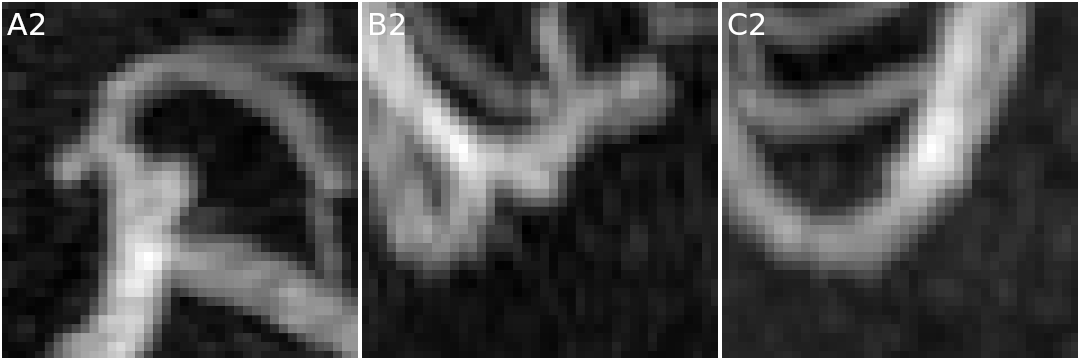
\includegraphics[width=\linewidth]{figures/mip_patch10028.png}
	\end{subfigure}
	\caption[Maximum Intensity Projections of two positive cases.]{\todo{caption}}
	\label{fig:mip_patch}
\end{figure}


As discussed in chapter \ref{chapter3}, the size of aneurysms in a TOF-MRA is very small; the mean diameter of an aneurysm in our dataset being $4.11$ mm. With a re-sampled volume with voxel spacing $0.3 \times 0.3 \times 0.3$ mm\textsuperscript{3}, the mean shape of a volume encompassing an aneurysm would be $21.5 \times 21.5 \times 21.5$ -- assuming a spherical structure of the aneurysm. Axial, coronal and sagittal images (after preprocessing of the TOF-MRA volumes) would have shapes $512 \times 512$, $512 \times 140$, and $512 \times 140$ respectively. Due to this, an MIP taken of the whole three-dimensional TOF-MRA volume, would have little useful information regarding the aneurysm, such as an enlarged vessel. Therefore, as most other training procedures for other networks, Triplanar-Net is trained using patches of the whole volume. MIPs are then taken for the patch of cropped volume, further allowing the network to learn important features with respect to the aneurysm segmentation such as structure and shape. The projections the network learns from are thus as in figure \ref{fig:mip_patch}, which are obtained from cropping a TOF-MRA volume centered around the aneurysm. \todo{Talk about ratio of patches} \todo{Why only positive patches?} \todo{What using only positive patches leads to}.

\todo{is it ok to use MIP as projection method for brain volumes and why, what might be lost using 2D images etc}


\section{Network architecture}
\todo{Figure for network architecture}

\img{trinet.png}{\linewidth}{\todo{caption}}{TriPlanar-Net architecture.}

\todo{Explain different parts}

\todo{2D MIPs only used as input, however 3D reconstruction is done within network, why? Why use 3D labels for training instead of 2D MIPs? State that since 3D binary labels would be needed as output, instead of reconstructing the volume from three 2D binary labels, it is more effective to reconstruct volume with intermediate representation of the three projections, and obtain 3D binary label after deconvolution.}

\todo{Math for 2D to 3D reconstruction?}

\todo{Downsides, and why the added step of classification before each patch should be added for inference.}

\todo{Advantages over other networks}

\section{Complete workflow}
\todo{Workflow including classification, preprocessing, processing}

\section{Inference}
\todo{Maybe remove section and add in complete workflow}
\todo{Talk about way to infer, math and shit maybe about 3D reconstruction}


